
\subsubsection{Problem definition}

The top and the bottom of a solid body that consists of one homogeneous material are heated. The $xy$-plane is the horizontal plane. The height of the body is in $z$-direction. The dimensions of this 3~D-model are 10~m in all directions. As deformations in $x$- and $y$-direction are suppressed, the increasing temperature evokes stresses within the solid. The aim of the calculation is to find out the isotropic state of stress that is reached after the whole solid is heated. Fig. \ref{fig61} shows a sketch of the calculation area.

\begin{figure}[htbp]
\centering
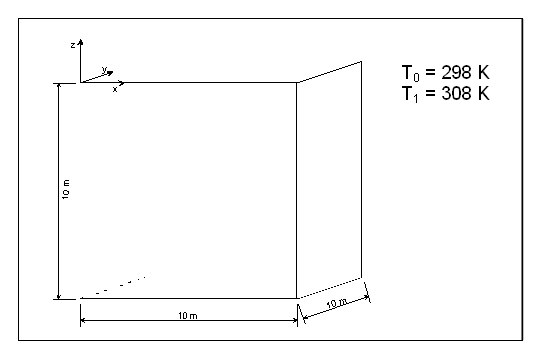
\includegraphics[width=0.6\textwidth]{TM/figures/fig61.eps}
\caption{Calculation area with one material}
\label{fig61}
\end{figure}

%\newpage

\textsl{Assumptions}

\begin{tabbing}
\=xxxxxxxxxxxx  \=xxxxxxxxxxxxxxxxxxxxxxx \kill
\> Temperature: \> constant temperature in the whole body at the beginning, heating \\
\> \> of the body about 10~K \\[1.0ex]
\> Solid: \> homogeneous, anisotropic, finite dimensions, no deformation at the \\
\> \> boundaries, linear elastic material behaviour, isotropic thermal ex- \\
\> \> pansion, different thermal expansion for the materials
\end{tabbing}

\subsubsection{Model set-up of the 3~D numerical model}

The dimensions of this 3~D-model are 10~m in all directions. Deformations perpendicular to the outer surfaces are suppressed. The initial temperature in the whole area is 298~K. At the top and at the bottom of the model thermal boundary conditions are set with a temperature of 308~K. Thereby the heating of the solid about 10~K is simulated. The used parameters of the solid represent the material behaviour of concrete (Tab. \ref{tab61}). 1000 elements and 1331 nodes are used. The calculation is divided in 384 time steps with a constant time step length of 900 seconds. That means the heating of the solid within 4 days is simulated. The calculation model is sketched in Fig. \ref{fig62}.
\begin{table}[htbp]
\centering
\begin{tabular}{|c|l|l|}
\hline
symbol & quantity & value \\
\hline
$T_0$  & Initial temperature (before heating) & 298 K \\
\hline
$T_1$  & Temperature after heating & 308 K \\
\hline
$\rho$  & Density of the solid &  2.2 t$\cdot$m$^{-3}$  \\			
\hline
$E$ & Young's modulus of the solid & 25 GPa \\
\hline
$\nu$ & Poisson ratio & 0.27 \\
\hline
$\alpha$ & Thermal expansion & 6.0$\cdot$10$^{-6}$ K$^{-1}$ \\
\hline
$c$      & Thermal capacity & 1.0 J$\cdot$kg$^{-1}\cdot$K$^{-1}$ \\
\hline
$\kappa$ & Thermal conductivity & 1.0 W$\cdot$m$^{-1}\cdot$K$^{-1}$ \\
\hline
\end{tabular}
\caption{Used parameters}
\label{tab61}
\end{table}

\begin{figure}[htbp]
\centering
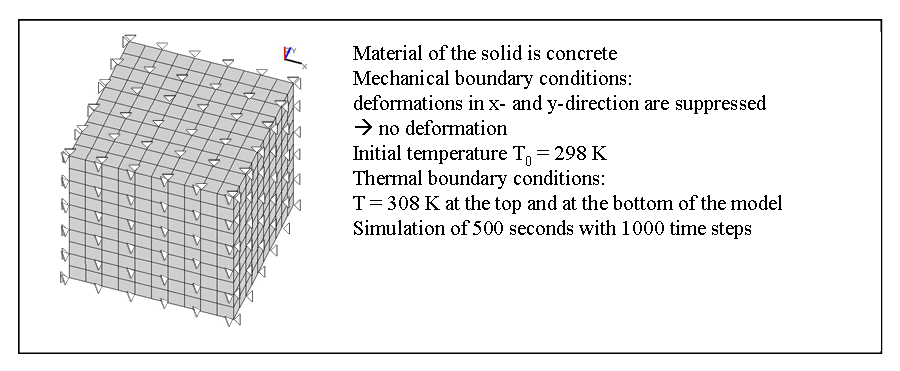
\includegraphics[width=0.9\textwidth]{TM/figures/fig62.eps}
\caption{Calculation model (3~D)}
\label{fig62}
\end{figure}

%\newpage

\subsubsection{Evaluation method}

The analytical solution can be derived from the time independent Eqns. \ref{eq61} to \ref{eq63} with the assumptions of no deformation and an isotropic thermal expansion:
\begin{eqnarray}
\varepsilon_i & \equiv & 0 \nonumber \\[1.5ex]
\sigma_x & = & \sigma_y\,=\,\sigma_z\,=\,
-\frac{\alpha\cdot\Delta T\cdot E}{1-2\cdot\nu}
\label{eq64}
\end{eqnarray}
Eqn. \ref{eq64} provides the stresses after heating the solid and shows an isotropic state of stress.

\subsubsection{Results}

With the analytical solution in Eqn. \ref{eq64} and the used parameters the stress values in the solid amount. This isotropic state of stress is reached after the whole solid is heated. The temporal development of the stresses in the centre of the model (at node 665) calculated is presented in Fig. \ref{fig63}. The results of the 3~D simulation show an exact agreement with the analytical solutions.

\begin{figure}[htbp]
\centering
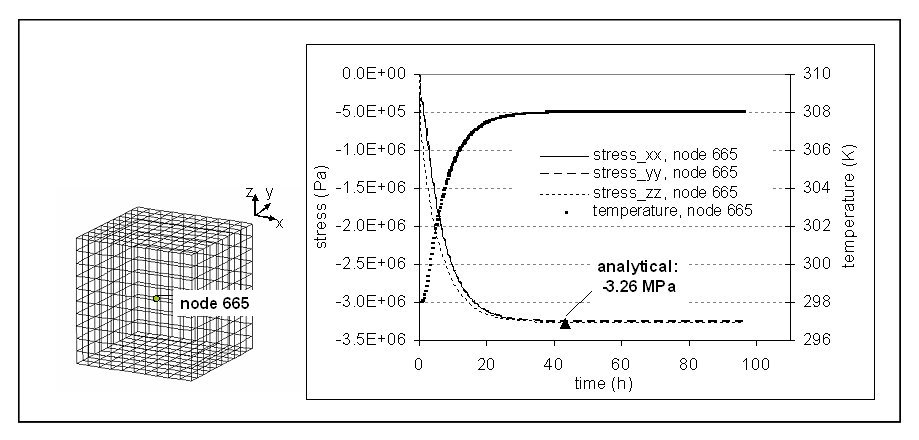
\includegraphics[width=0.9\textwidth]{TM/figures/fig63.eps}
\caption{Temporal stress development in the centre of the calculation model (node 665)}
\label{fig63}
\end{figure}

\begin{tabular}{|l|l|l|l|}
\hline
Path in the & Used code	& Used version & Date of simu- \\
benchmark deposit	& & & lation run \\
\hline	
TM$\backslash$heating$\backslash$cube$\backslash$	& GeoSys/RockFlow	& RockFlow 4,	rf4 & Dec. 2007 \\
tm\_01\_3Du	& & 4.05.07 & \\
\hline	
\end{tabular}
